\documentclass[a4paper,12pt]{article}
\usepackage[utf8]{inputenc}
\usepackage[spanish]{babel}
\usepackage{color}
\usepackage{parskip}
\usepackage{graphicx}
\usepackage{multirow}
\usepackage{listings}
\usepackage{vmargin}
\usepackage{datetime}
\newdate{date}{9}{11}{2017}
\graphicspath{ {imagenes/} }
\definecolor{mygreen}{rgb}{0,0.6,0}
\definecolor{lbcolor}{rgb}{0.9,0.9,0.9}
\usepackage{epstopdf}
\usepackage{float}


\setpapersize{A4}
\setmargins{2.5cm}       % margen izquierdo
{1.5cm}                        % margen superior
{16.5cm}                      % anchura del texto
{23.42cm}                    % altura del texto
{10pt}                           % altura de los encabezados
{1cm}                           % espacio entre el texto y los encabezados
{0pt}                             % altura del pie de página
{2cm}     

\lstset{
    tabsize=4,    
%   rulecolor=,
    language=[GNU]C++,
        basicstyle=\tiny,
        aboveskip={1.5\baselineskip},
        columns=fixed,
        showstringspaces=false,
        extendedchars=false,
        breaklines=true,
        prebreak = \raisebox{0ex}[0ex][0ex]{\ensuremath{\hookleftarrow}},
        frame=single,
        showtabs=false,
        showspaces=false,
        showstringspaces=false,
        identifierstyle=\ttfamily,
        keywordstyle=\color[rgb]{0,0,1},
        commentstyle=\color[rgb]{0.026,0.112,0.095},
        stringstyle=\color{red},
        numberstyle=\color[rgb]{0.205, 0.142, 0.73},
%        \lstdefinestyle{C++}{language=C++,style=numbers}’.
}


\begin{document}
\title{Práctica de Laboratorio 4}
\author{
Christofer Fabián Chávez Carazas \\
\small{Universidad Nacional de San Agustín de Arequipa} \\
\small{Escuela Profesional de Ciencia de la Computación} \\
\small{Computación Gráfica}
}
\date{\displaydate{date}}

\maketitle

\begin{large}
 \textbf{Desarrolle el siguiente programa}
\end{large}

Implemente un programa de una versión primitiva del PaintBrush, el cual e permita dibujar líneas, círculos, cuadrados y elipses con el mouse. El programa debe capturar la posición
x,y al presionar el mouse y mientras se arrastra debe dibujar la figura hasta la posición en la que se mueve el puntero. Al soltar debe quedar la figura.
Se recomienda para este ejercicio que se defina un modelo con un sistema de coordenadas similar al de la pantalla, para no tener que traducir coordenadas del modelo a la
pantalla. Al pintar una segunda figura no es necesario que se mantenga el primero. El cambio de figura y/o color debe ser por medio de un menú.

\begin{large}
 \textbf{Programa}
\end{large}

Todas las primitivas usadas para pintar los diferentes dibujos son las funciones hechas por mí en anteriores prácticas. Todas las figuras se dibujan en base
a dos puntos: \textit{inicial} y \textit{final}. El programa detecta si el click está presionado o no según la variable global \textit{mouseState}. Cuando el click es
presionado por primera vez, las coordenadas del punto se guardan en la estructura \textit{inicial}. Mientras el click se mantiene presionado, las coordenadas que se
capturan se guardan en la estructura \textit{final}

\begin{lstlisting}
#include <GL/glut.h>
#include <iostream>
#include "primitivas.h"

using namespace std;

int windowWidth = 400;
int windowHeight = 400;

Window window;

int iFondo = 0;
int iDibujo = 3;
int poligono = 0;
int mouseX = 0;
int mouseY = 0;
int mouseState = -1;

Point inicial;
Point final;

typedef enum {FONDO1, FONDO2, FONDO3, DIBUJO1, DIBUJO2, DIBUJO3, LINEA, RECTANGULO, CIRCULO, ELIPSE} opcionesMenu;
enum MouseStates {DOWN, UP};

void onMenu(int option){
    switch(option){
        case FONDO1: iFondo = 0; break;
        case FONDO2: iFondo = 1; break;
        case FONDO3: iFondo = 2; break;
        case DIBUJO1: iDibujo = 3; break;
        case DIBUJO2: iDibujo = 4; break;
        case DIBUJO3: iDibujo = 5; break;
        case LINEA: poligono = 6; break;
        case RECTANGULO: poligono = 7; break;
        case CIRCULO: poligono = 8; break;
        case ELIPSE: poligono = 9; break;
    }
    glutPostRedisplay();
}

void creationMenu(){
    int menuFondo, menuDibujo, menuPoligono, menuPrincipal;

    menuFondo = glutCreateMenu(onMenu);
    glutAddMenuEntry("Blanco", FONDO1);
    glutAddMenuEntry("Verde Claro", FONDO2);
    glutAddMenuEntry("Azul Claro", FONDO3);

    menuDibujo = glutCreateMenu(onMenu);
    glutAddMenuEntry("Negro", DIBUJO1);
    glutAddMenuEntry("Verde Oscuro", DIBUJO2);
    glutAddMenuEntry("Azul Oscuro", DIBUJO3);

    menuPoligono = glutCreateMenu(onMenu);
    glutAddMenuEntry("Linea", LINEA);
    glutAddMenuEntry("Rectangulo", RECTANGULO);
    glutAddMenuEntry("Circulo", CIRCULO);
    glutAddMenuEntry("Elipse", ELIPSE);

    menuPrincipal = glutCreateMenu(onMenu);
    glutAddSubMenu("Color de fondo", menuFondo);
    glutAddSubMenu("Color de dibujo", menuDibujo);
    glutAddSubMenu("Poligono", menuPoligono);
    glutAttachMenu(GLUT_RIGHT_BUTTON);
}

void resize(GLsizei w, GLsizei h){
    windowWidth = w;
    windowHeight = h;
    glViewport(0,0, w, h);
    glMatrixMode(GL_PROJECTION);
    glLoadIdentity();
    glOrtho(0, w, 0, h, 1.f, -1.f);
    glMatrixMode(GL_MODELVIEW);
    glLoadIdentity();
}

void mouse_move(int x, int y){
    mouseX = x;
    mouseY = windowHeight - y;
    if(mouseState == DOWN){
        final.x = mouseX;
        final.y = mouseY;
    }
    glutPostRedisplay();
}

void mouse_drag(int x, int y){
    mouseX = x;
    mouseY = windowHeight - y;
    if(mouseState == DOWN){
        final.x = mouseX;
        final.y = mouseY;
    }
    glutPostRedisplay();
}

void mouse_click(int button, int state, int x, int y){
    if(button == GLUT_LEFT_BUTTON){
        if(state == GLUT_UP){
            mouseState = UP;
        }
        else if(state == GLUT_DOWN){
            mouseState = DOWN;
            inicial.x = mouseX;
            inicial.y = mouseY;
        }
        
    }
}

void timer_function(int value){
    glutTimerFunc(8000, timer_function, 1);
}

void display(){
    float colores[6][3] = {
        { 1.00f, 1.00f, 1.00f},
        { 0.12f, 0.50f, 0.26f},
        { 0.20f, 0.14f, 0.66f},
        { 0.00f, 0.00f, 0.00f},
        { 0.06f, 0.25f, 0.13f},
        { 0.10f, 0.07f, 0.33f}
    };

    glClearColor(colores[iFondo][0], colores[iFondo][1], colores[iFondo][2], 1.0f);
    glClear(GL_COLOR_BUFFER_BIT);
    glColor3f(colores[iDibujo][0], colores[iDibujo][1], colores[iDibujo][2]);

    switch(poligono){
        case LINEA: drawLineXnpio(inicial, final, window); break;
        case RECTANGULO: drawRectangle(inicial, final, window); break;
        case CIRCULO: {
            Point centroCirc;
            GLint radius = max(abs(inicial.x - final.x), abs(inicial.y - final.y)) / 2;
            centroCirc.x = min(inicial.x, final.x) + radius;
            centroCirc.y = min(inicial.y, final.y) + radius;
            circleMidPoint(centroCirc, radius, window);
            break;
        }
        case ELIPSE: {
            Point centroElip;
            GLint radiusX = abs(inicial.x - final.x) / 2;
            GLint radiusY = abs(inicial.y - final.y) / 2;
            centroElip.x = min(inicial.x, final.x) + radiusX;
            centroElip.y = min(inicial.y, final.y) + radiusY;
            elipceMidPoint(centroElip, radiusX, radiusY, window);
            break;
        }
        default: break;
        
    }
    glFlush();
    glutSwapBuffers();
}

int main(int argc, char **argv){
    window.height = windowHeight;
    window.width = windowWidth;
    inicial.x = windowHeight;
    inicial.y = windowWidth;
    final.x = windowHeight;
    final.y = windowWidth;
    glutInit(&argc, argv);
    glutInitDisplayMode(GLUT_DOUBLE | GLUT_RGB | GLUT_DEPTH);
    glutInitWindowSize(windowHeight, windowWidth);
    glutInitWindowPosition(100, 100);
    glutCreateWindow("PaintBrush");
    glutDisplayFunc(display);
    glutReshapeFunc(resize);
    glutPassiveMotionFunc(mouse_move);
    glutMotionFunc(mouse_drag);
    glutMouseFunc(mouse_click);
    glutTimerFunc(33, timer_function, 1);
    creationMenu();
    glutMainLoop();
    return 0;
}
\end{lstlisting}

\begin{large}
 \textbf{Resultados}
\end{large}


\begin{figure}[H]
 \centering
 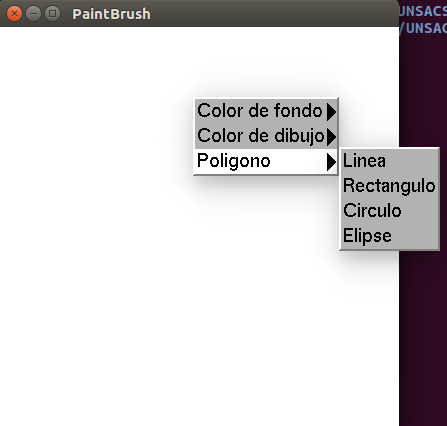
\includegraphics[scale = 0.5]{1.png}
 \caption{Menús}
\end{figure}
\begin{figure}[H]
 \centering
 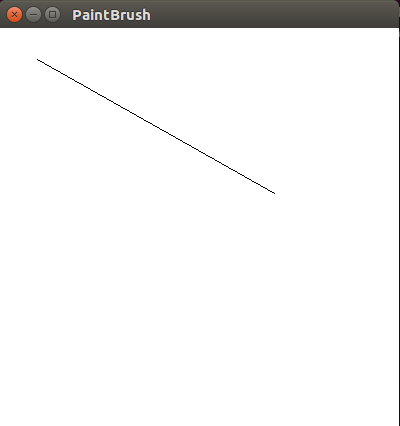
\includegraphics[scale = 0.5]{2.png}
 \caption{Línea}
\end{figure}
\begin{figure}[H]
 \centering
 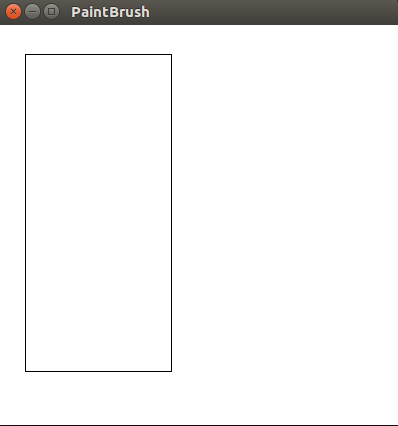
\includegraphics[scale = 0.5]{3.png}
 \caption{Rectángulo}
\end{figure}
\begin{figure}[H]
 \centering
 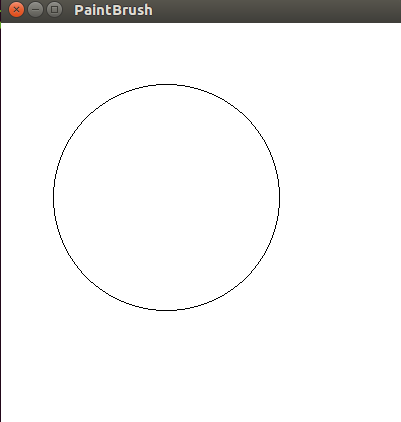
\includegraphics[scale = 0.5]{4.png}
 \caption{Círculo}
\end{figure}
\begin{figure}[H]
 \centering
 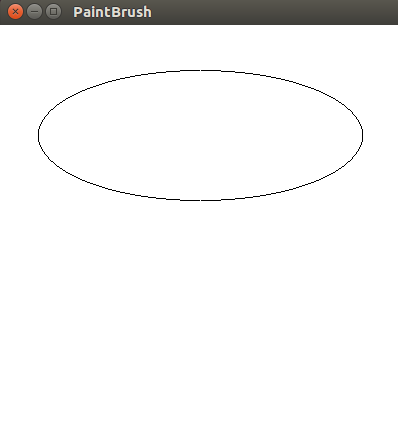
\includegraphics[scale = 0.5]{5.png}
 \caption{Elipse}
\end{figure}




\end{document}

